%%%%%%%%%%%%%%%%%%%%%%%%%%%%%%%%%%%%%%%%%%%%%%%%%%%%%%%%%%%%%%%%%%%%%%%%%%%%%%%%%%
\begin{frame}[fragile]\frametitle{}

\begin{center}
{\Large Parts-of-speech (PoS) in spaCy}

{\tiny (Ref:https://spacy.io/usage/linguistic-features)}

\end{center}


\end{frame}

%%%%%%%%%%%%%%%%%%%%%%%%%%%%%%%%%%%%%%%%%%%%%%%%%%%%%%%%%%%%%%%%%%%%%%%%%%%%%%%%%%
\begin{frame}[fragile]\frametitle{Part-of-speech tagging}
  \begin{itemize}
    \item After tokenization, spaCy can parse and tag a given Doc
		\item Makes a prediction of which tag or label most likely applies
  \end{itemize}
	
\end{frame}

%%%%%%%%%%%%%%%%%%%%%%%%%%%%%%%%%%%%%%%%%%%%%%%%%%%%%%%%%%%%%%%%%%%%%%%%%%%%%%%%%%
\begin{frame}[fragile]\frametitle{Parts of Speech [POS] Tagging }

\begin{lstlisting}
text = 'Apple is looking for buying a U.K. startup. Government has given permission.'

doc = nlp(text)
print(doc)

>> Apple is looking for buying a U.K. startup for $1 billion

for token in doc:
    print(token.text, token.pos_)

Apple PROPN
is AUX
looking VERB
for ADP
buying VERB
a DET
U.K. PROPN
startup NOUN
for ADP
$ SYM
1 NUM
billion NUM
\end{lstlisting}
	
\end{frame}

%%%%%%%%%%%%%%%%%%%%%%%%%%%%%%%%%%%%%%%%%%%%%%%%%%%%%%%%%%%%%%%%%%%%%%%%%%%%%%%%%%
\begin{frame}[fragile]\frametitle{Results}
	
\begin{center}
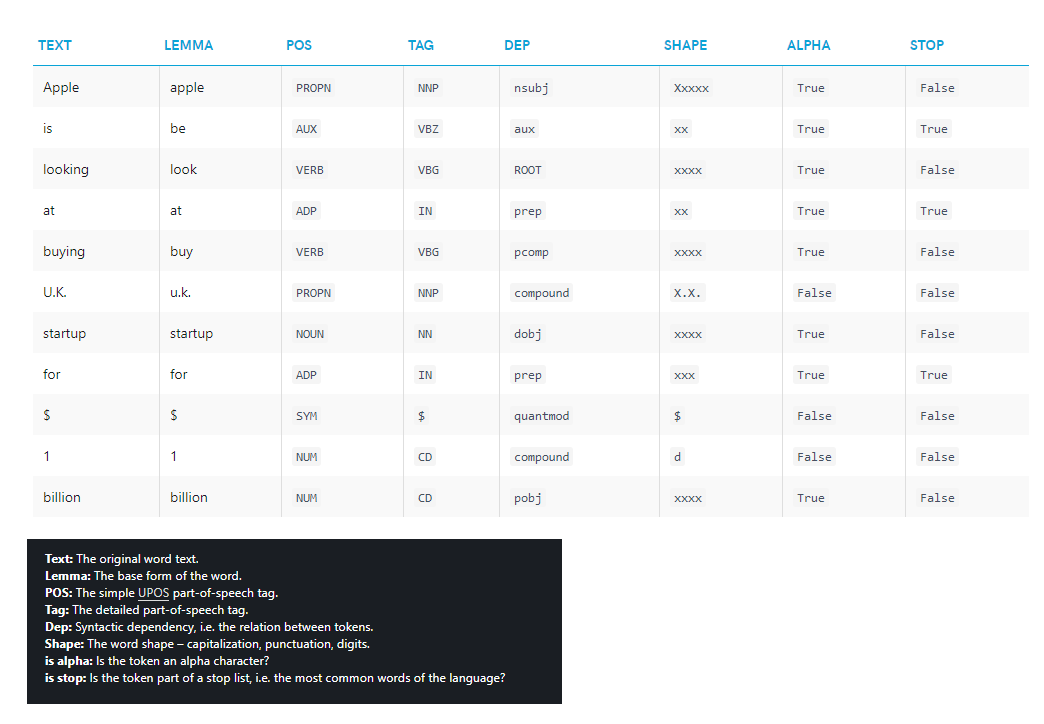
\includegraphics[width=\linewidth,keepaspectratio]{spacy11}
\end{center}

\end{frame}

%%%%%%%%%%%%%%%%%%%%%%%%%%%%%%%%%%%%%%%%%%%%%%%%%%%%%%%%%%%%%%%%%%%%%%%%%%%%%%%%%%
\begin{frame}[fragile]\frametitle{Dependency Parsing}

\begin{lstlisting}
from spacy import displacy

nlp = spacy.load("en_core_web_sm")
doc = nlp("This is a sentence.")
displacy.serve(doc, style="dep")
\end{lstlisting}

\begin{center}
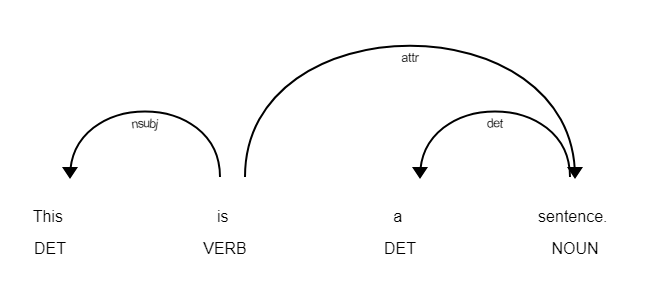
\includegraphics[width=0.4\linewidth,keepaspectratio]{spacy12}
\end{center}

\begin{lstlisting}
options = {"compact": True, "bg": "#09a3d5",
           "color": "white", "font": "Source Sans Pro"}
displacy.serve(doc, style="dep", options=options)
\end{lstlisting}

\begin{center}
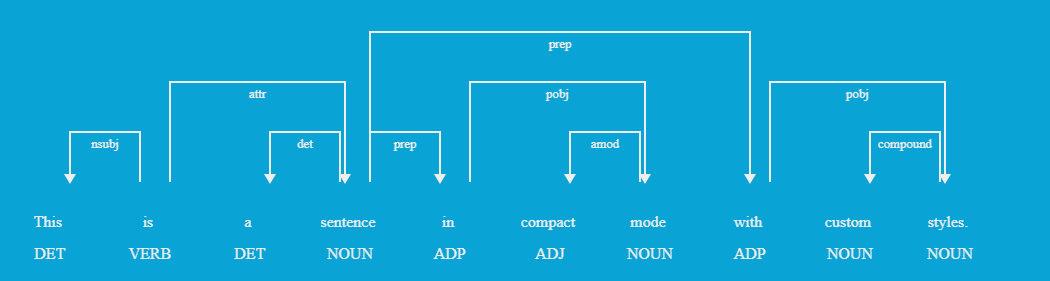
\includegraphics[width=0.6\linewidth,keepaspectratio]{spacy13}
\end{center}

\end{frame}


%%%%%%%%%%%%%%%%%%%%%%%%%%%%%%%%%%%%%%%%%%%%%%%%%%%%%%%%%%%%%%%%%%%%%%%%%%%%%%%%%%
\begin{frame}[fragile]\frametitle{Exercise}

  \begin{itemize}
    \item Process the text with the nlp object and create a doc.
    \item For each token, print the token text, the token's .pos\_ (part-of-speech tag) and the token's .dep\_ (dependency label).
  \end{itemize}

  \begin{lstlisting}
import spacy

nlp = spacy.load("en_core_web_sm")

text = "It's official: Apple is the first U.S. public company to reach a $1 trillion market value"

# Process the text
doc = ____

for token in doc:
    # Get the token text, part-of-speech tag and dependency label
    token_text = ____.____
    token_pos = ____.____
    token_dep = ____.____
    # This is for formatting only
    print(f"{token_text:<12}{token_pos:<10}{token_dep:<10}")
  \end{lstlisting}
	
\end{frame}